\documentclass{standalone}
\usepackage{tikz}
\begin{document}
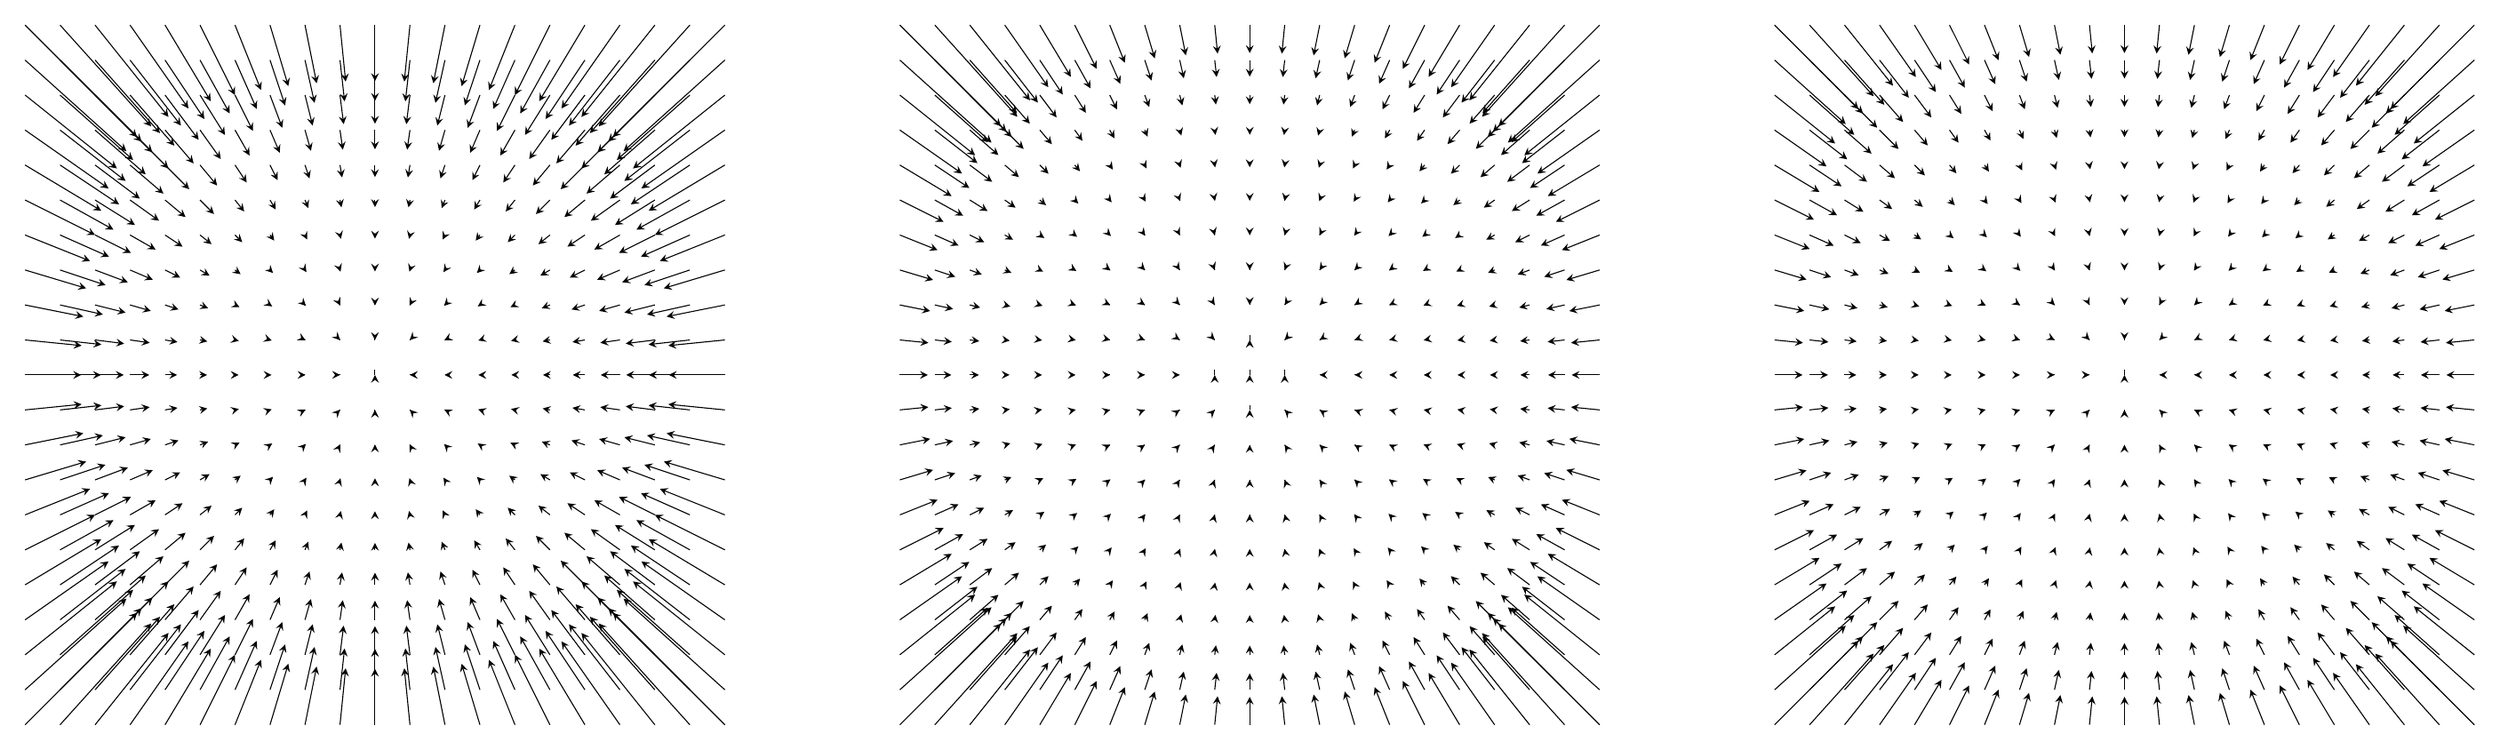
\begin{tikzpicture}[scale=5]

\newcommand*{\render}[2]{
	\foreach \y in {-10,...,10} {
		\foreach \x in {-10,...,10} {
		\def\xx{(\x/10)}
		\def\yy{(\y/10)}

		\def\rr{(\xx*\xx+\yy*\yy)}

		\def\corr{(1.0+#1*\rr+#2*\rr*\rr)}
		\def\xd{\xx*\corr}
		\def\yd{\yy*\corr}

		%\draw ({\xx},{\yy}) -- ({\xd},{\yd});
		\draw [-stealth] ({\xx},{\yy}) -- ({\xd},{\yd});
		}
	}
}

\render{-0.16}{0.00}

\begin{scope}[xshift = 2.5cm]
	\render{0.00}{-0.08}
\end{scope}

\begin{scope}[xshift = 5cm]
	\render{-0.04}{-0.04}
\end{scope}

\end{tikzpicture}
\end{document}
